\documentclass[12pt,letterpaper]{article}
\usepackage[utf8]{inputenc}
\usepackage[spanish]{babel}
\usepackage{graphicx}
\usepackage{tabularx}
\usepackage{multirow}
\usepackage{float}
\usepackage{hyperref}
\usepackage{enumerate} 

\begin{document}
\begin{center}
{\Large \textbf{Métodos Computacionales - Taller 5}}\\
\vspace{0.3cm}
\textbf{Julián Leandro Rodríguez Cardona - 201416065}\\ \vspace{0.3cm}
\end{center}

\section*{Métodos de Monte Carlo}

Se presentan los resultados.

\section{Canales iónicos}

\begin{figure}[H]
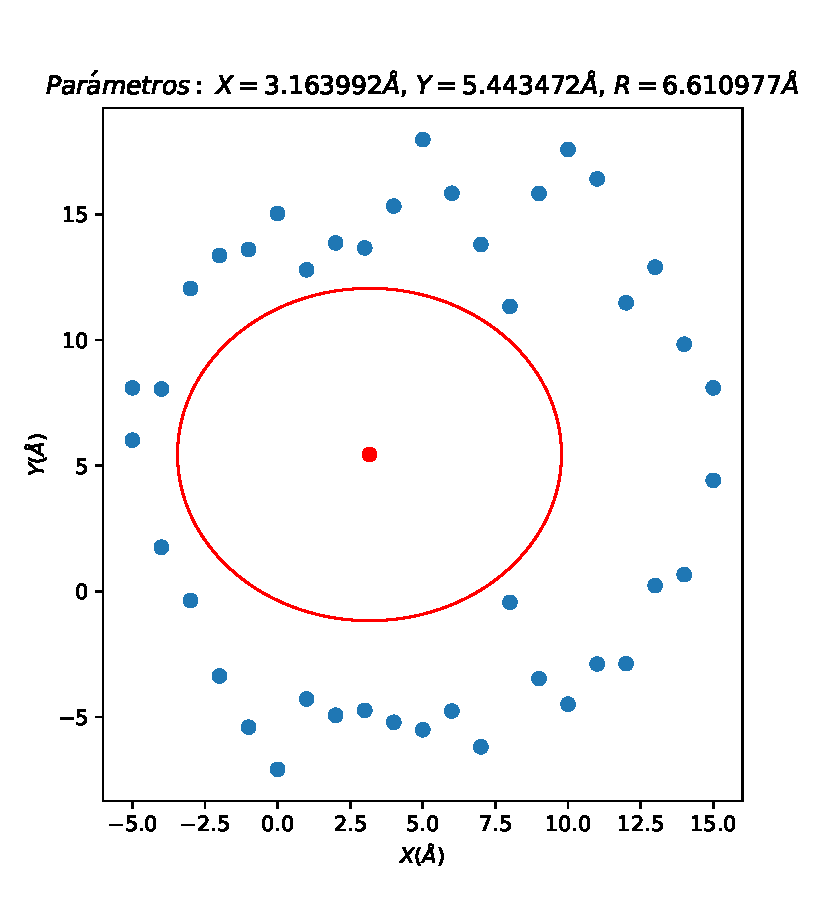
\includegraphics{canal.pdf}
\caption{Circulo de máximo radio en el canal del archivo "Canal\_ionico.txt".}
\centering
\end{figure}

\begin{figure}[H]
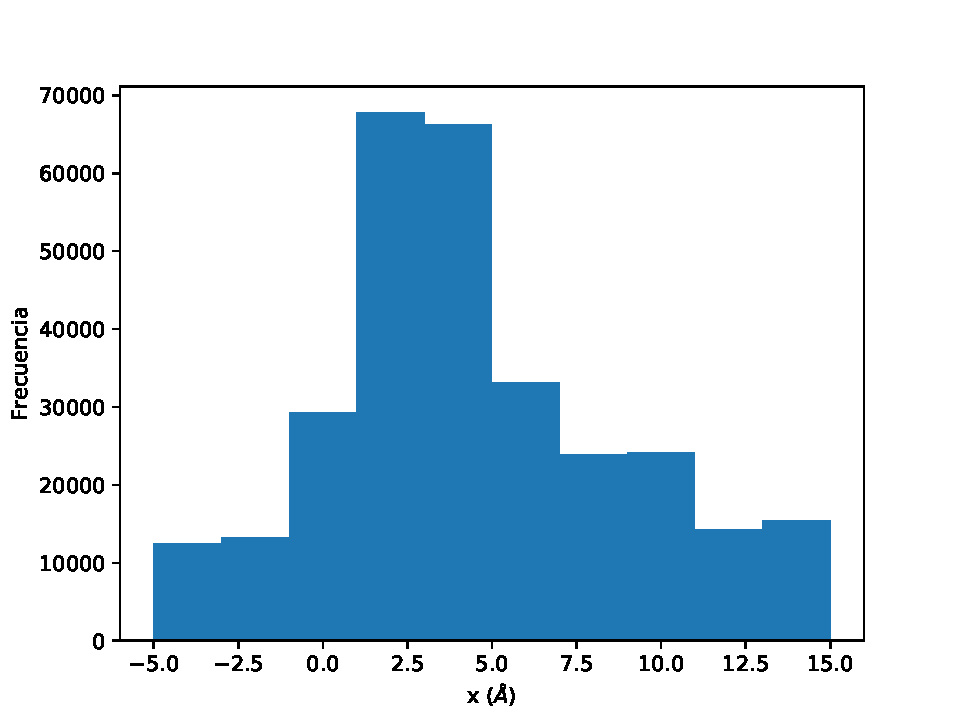
\includegraphics{x_hist.pdf}
\caption{Histograma de la coordenada x.}
\centering
\end{figure}

\begin{figure}[H]
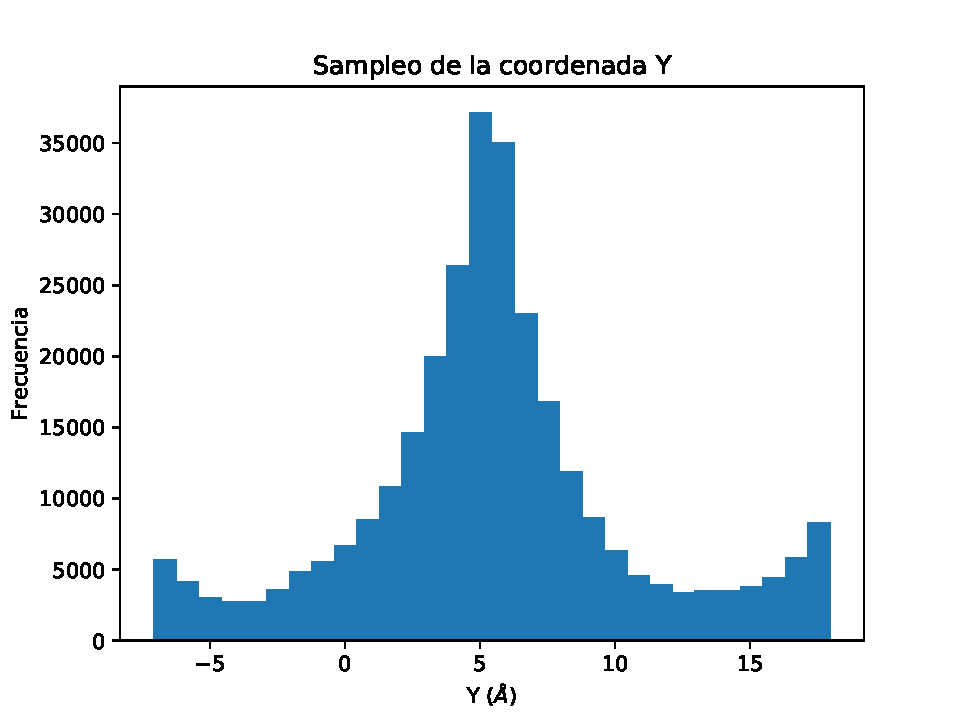
\includegraphics{y_hist.pdf}
\caption{Histograma de la coordenada y.}
\centering
\end{figure}


\begin{figure}[H]
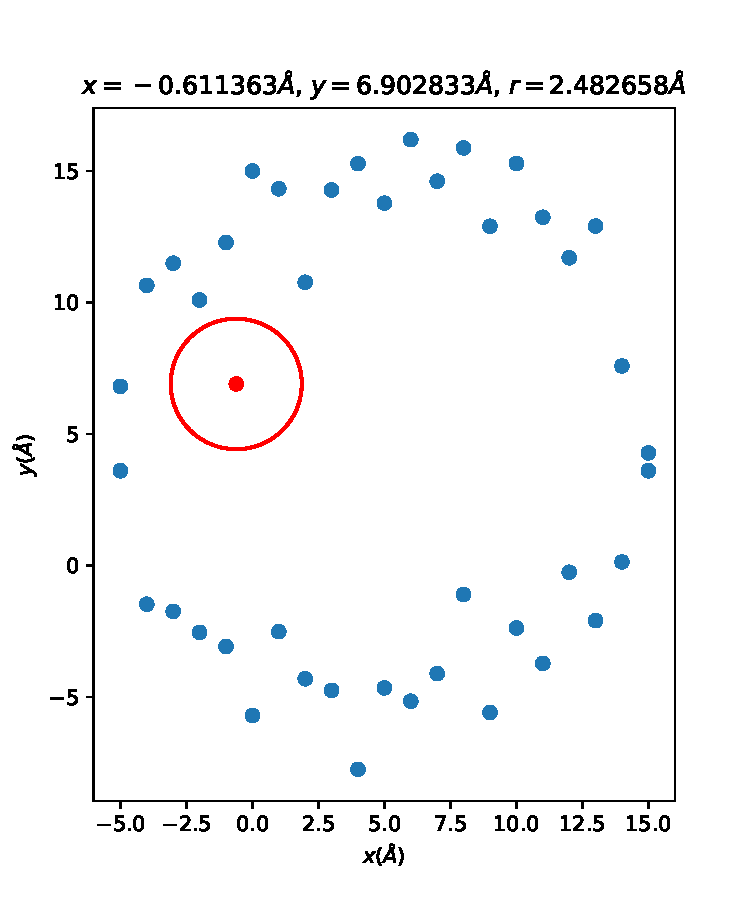
\includegraphics{canal1.pdf}
\caption{Circulo de máximo radio en el canal del archivo "Canal\_ionico1.txt".}
\centering
\end{figure}

\begin{figure}[H]
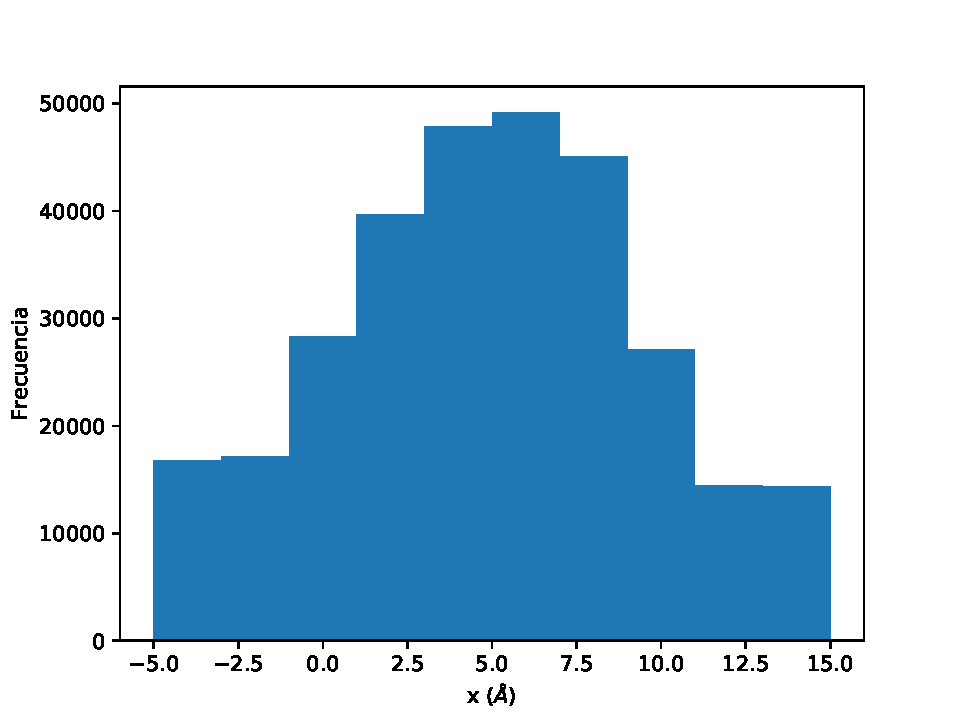
\includegraphics{x1_hist.pdf}
\caption{Histograma de la coordenada x.}
\centering
\end{figure}

\begin{figure}[H]
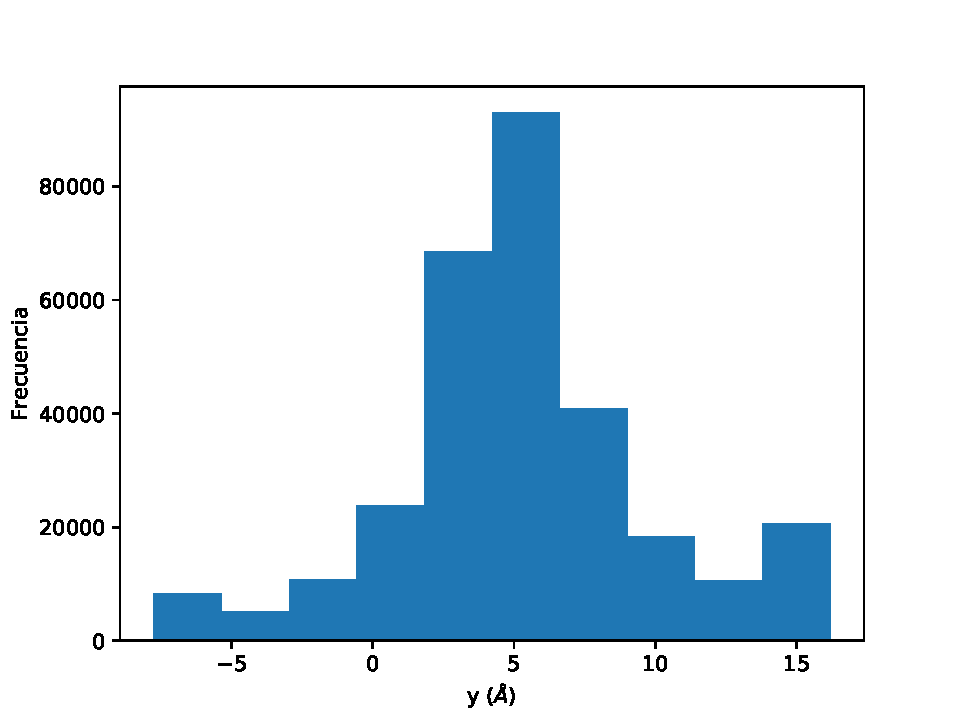
\includegraphics{y1_hist.pdf}
\caption{Histograma de la coordenada y.}
\centering
\end{figure}

\section{Circuito RC}

\subsection*{Resistencia}
\begin{figure}[H]
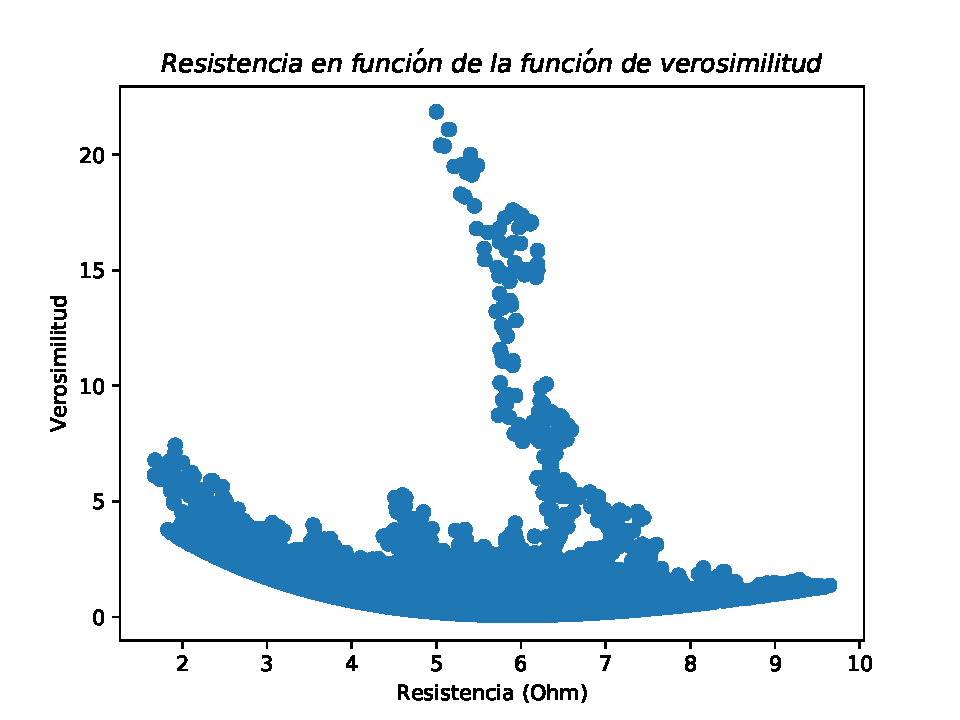
\includegraphics{r_verosimilitud.pdf}
\centering
\end{figure}

\begin{figure}[H]
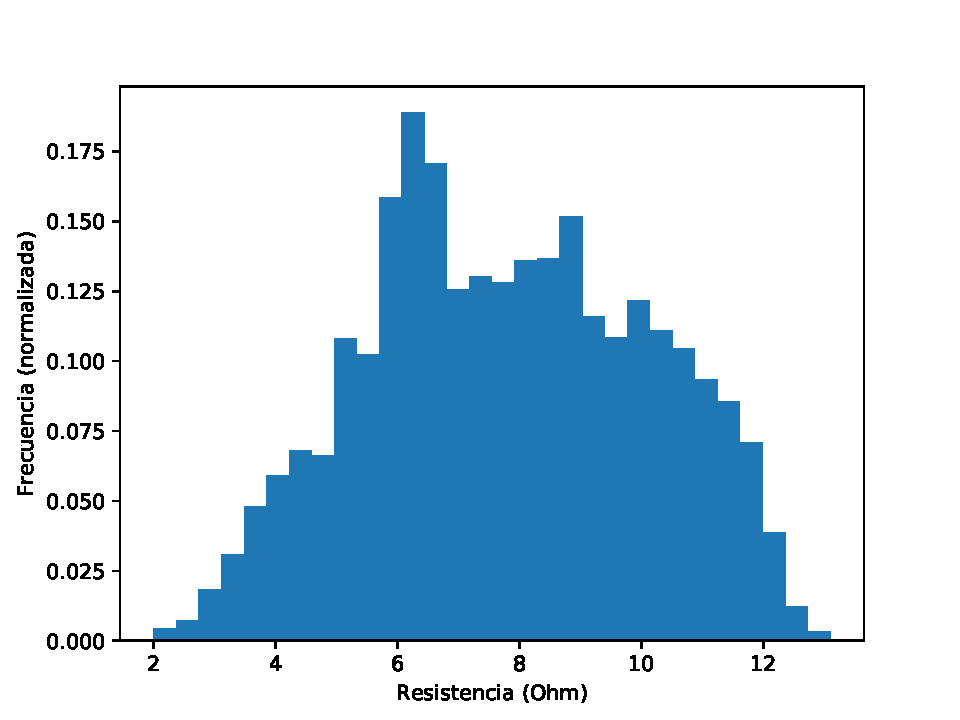
\includegraphics{r_hist.pdf}
\centering
\end{figure}

\subsection{Capacitancia}

\begin{figure}[H]
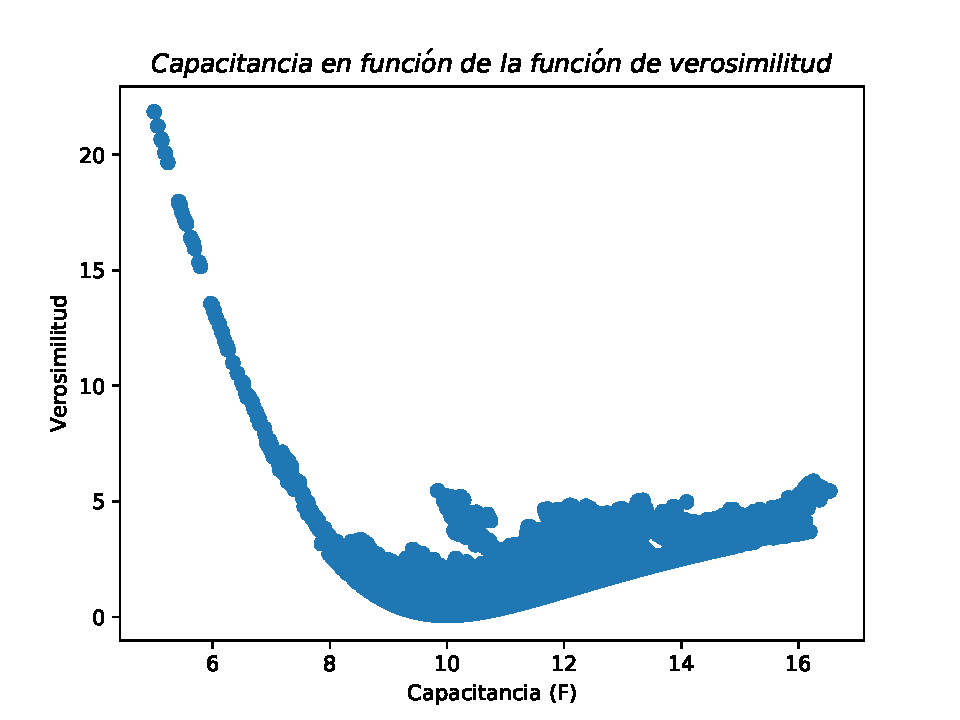
\includegraphics{c_verosimilitud.pdf}
\centering
\end{figure}

\begin{figure}[H]
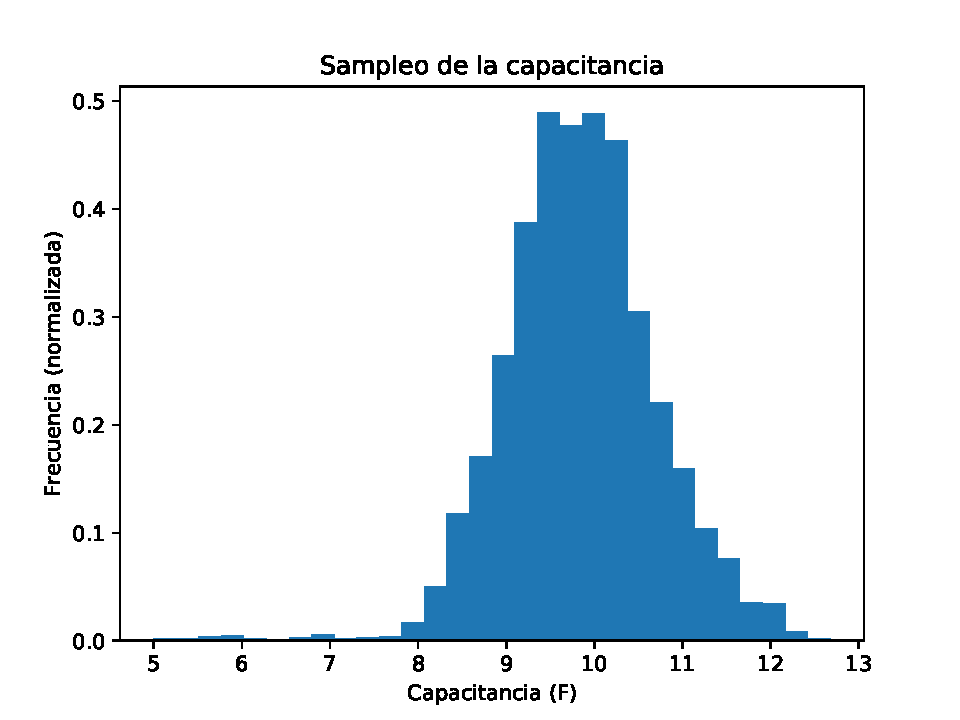
\includegraphics{c_hist.pdf}
\centering
\end{figure}

\subsection*{Carga en función del tiempo}
\begin{figure}[H]
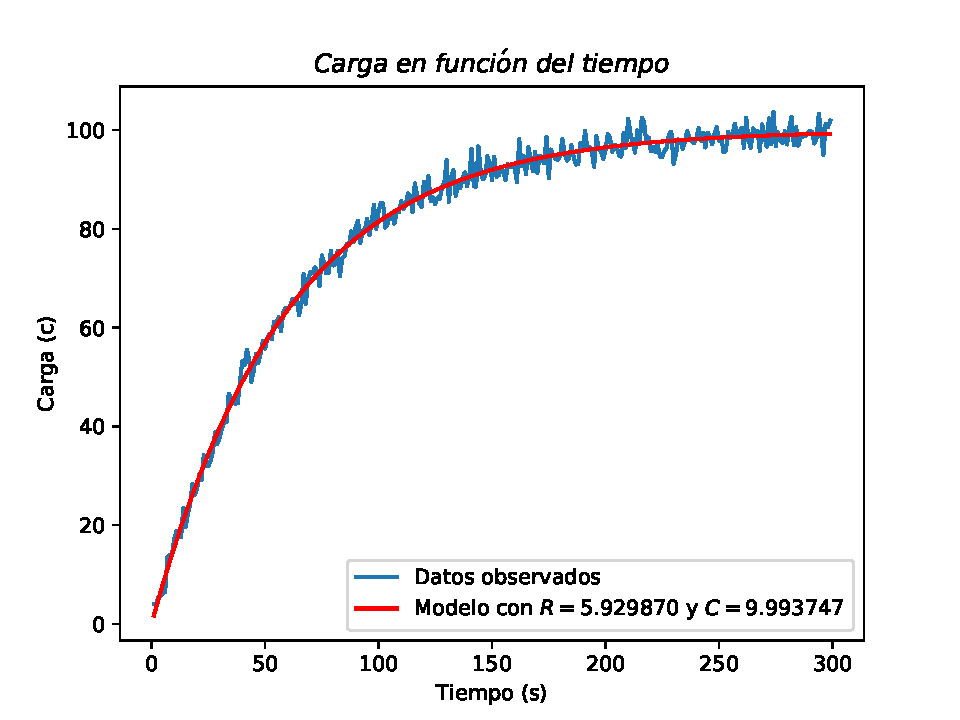
\includegraphics{carga.pdf}
\centering
\end{figure}

\vspace{0.3cm}


\end{document}
